% !TEX TS-program = pdflatex
% !TEX encoding = UTF-8 Unicode
\documentclass[border=0mm]{standalone}
% packages
\usepackage{tikz}
\usetikzlibrary{patterns}
\usepackage{amsmath,amssymb}
\usepackage{bm}
\usepackage{pgfplots}
\pgfplotsset{compat=1.15}
% start document
\begin{document}
% generated by ROOT (CERN)
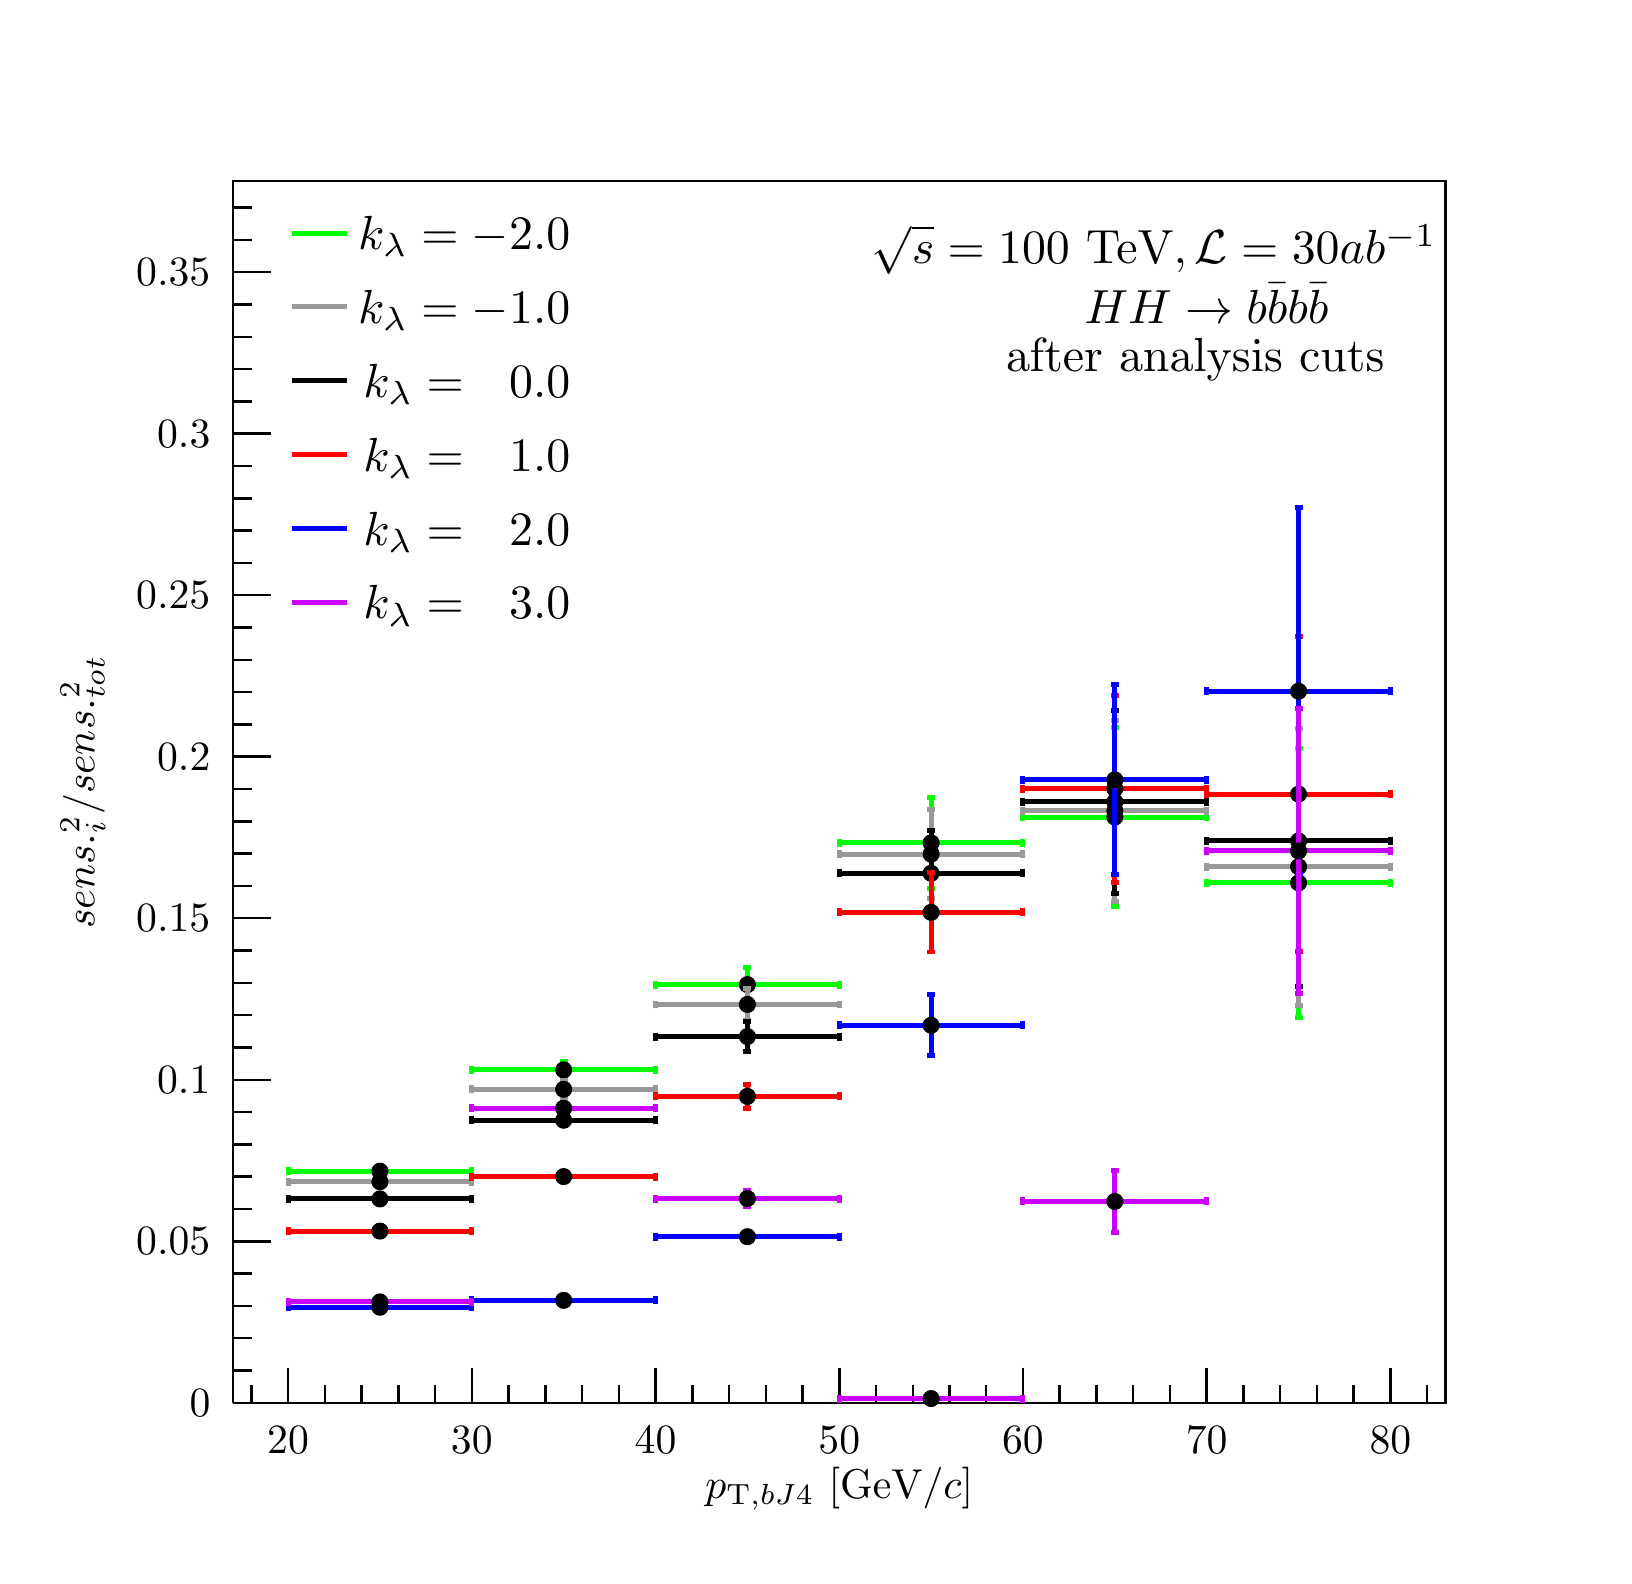
\begin{tikzpicture}
\pgfdeclareplotmark{cross} {
\pgfpathmoveto{\pgfpoint{-0.3\pgfplotmarksize}{\pgfplotmarksize}}
\pgfpathlineto{\pgfpoint{+0.3\pgfplotmarksize}{\pgfplotmarksize}}
\pgfpathlineto{\pgfpoint{+0.3\pgfplotmarksize}{0.3\pgfplotmarksize}}
\pgfpathlineto{\pgfpoint{+1\pgfplotmarksize}{0.3\pgfplotmarksize}}
\pgfpathlineto{\pgfpoint{+1\pgfplotmarksize}{-0.3\pgfplotmarksize}}
\pgfpathlineto{\pgfpoint{+0.3\pgfplotmarksize}{-0.3\pgfplotmarksize}}
\pgfpathlineto{\pgfpoint{+0.3\pgfplotmarksize}{-1.\pgfplotmarksize}}
\pgfpathlineto{\pgfpoint{-0.3\pgfplotmarksize}{-1.\pgfplotmarksize}}
\pgfpathlineto{\pgfpoint{-0.3\pgfplotmarksize}{-0.3\pgfplotmarksize}}
\pgfpathlineto{\pgfpoint{-1.\pgfplotmarksize}{-0.3\pgfplotmarksize}}
\pgfpathlineto{\pgfpoint{-1.\pgfplotmarksize}{0.3\pgfplotmarksize}}
\pgfpathlineto{\pgfpoint{-0.3\pgfplotmarksize}{0.3\pgfplotmarksize}}
\pgfpathclose
\pgfusepathqstroke
}
\pgfdeclareplotmark{cross*} {
\pgfpathmoveto{\pgfpoint{-0.3\pgfplotmarksize}{\pgfplotmarksize}}
\pgfpathlineto{\pgfpoint{+0.3\pgfplotmarksize}{\pgfplotmarksize}}
\pgfpathlineto{\pgfpoint{+0.3\pgfplotmarksize}{0.3\pgfplotmarksize}}
\pgfpathlineto{\pgfpoint{+1\pgfplotmarksize}{0.3\pgfplotmarksize}}
\pgfpathlineto{\pgfpoint{+1\pgfplotmarksize}{-0.3\pgfplotmarksize}}
\pgfpathlineto{\pgfpoint{+0.3\pgfplotmarksize}{-0.3\pgfplotmarksize}}
\pgfpathlineto{\pgfpoint{+0.3\pgfplotmarksize}{-1.\pgfplotmarksize}}
\pgfpathlineto{\pgfpoint{-0.3\pgfplotmarksize}{-1.\pgfplotmarksize}}
\pgfpathlineto{\pgfpoint{-0.3\pgfplotmarksize}{-0.3\pgfplotmarksize}}
\pgfpathlineto{\pgfpoint{-1.\pgfplotmarksize}{-0.3\pgfplotmarksize}}
\pgfpathlineto{\pgfpoint{-1.\pgfplotmarksize}{0.3\pgfplotmarksize}}
\pgfpathlineto{\pgfpoint{-0.3\pgfplotmarksize}{0.3\pgfplotmarksize}}
\pgfpathclose
\pgfusepathqfillstroke
}
\pgfdeclareplotmark{newstar} {
\pgfpathmoveto{\pgfqpoint{0pt}{\pgfplotmarksize}}
\pgfpathlineto{\pgfqpointpolar{44}{0.5\pgfplotmarksize}}
\pgfpathlineto{\pgfqpointpolar{18}{\pgfplotmarksize}}
\pgfpathlineto{\pgfqpointpolar{-20}{0.5\pgfplotmarksize}}
\pgfpathlineto{\pgfqpointpolar{-54}{\pgfplotmarksize}}
\pgfpathlineto{\pgfqpointpolar{-90}{0.5\pgfplotmarksize}}
\pgfpathlineto{\pgfqpointpolar{234}{\pgfplotmarksize}}
\pgfpathlineto{\pgfqpointpolar{198}{0.5\pgfplotmarksize}}
\pgfpathlineto{\pgfqpointpolar{162}{\pgfplotmarksize}}
\pgfpathlineto{\pgfqpointpolar{134}{0.5\pgfplotmarksize}}
\pgfpathclose
\pgfusepathqstroke
}
\pgfdeclareplotmark{newstar*} {
\pgfpathmoveto{\pgfqpoint{0pt}{\pgfplotmarksize}}
\pgfpathlineto{\pgfqpointpolar{44}{0.5\pgfplotmarksize}}
\pgfpathlineto{\pgfqpointpolar{18}{\pgfplotmarksize}}
\pgfpathlineto{\pgfqpointpolar{-20}{0.5\pgfplotmarksize}}
\pgfpathlineto{\pgfqpointpolar{-54}{\pgfplotmarksize}}
\pgfpathlineto{\pgfqpointpolar{-90}{0.5\pgfplotmarksize}}
\pgfpathlineto{\pgfqpointpolar{234}{\pgfplotmarksize}}
\pgfpathlineto{\pgfqpointpolar{198}{0.5\pgfplotmarksize}}
\pgfpathlineto{\pgfqpointpolar{162}{\pgfplotmarksize}}
\pgfpathlineto{\pgfqpointpolar{134}{0.5\pgfplotmarksize}}
\pgfpathclose
\pgfusepathqfillstroke
}
\definecolor{c}{rgb}{1,1,1};
\draw [color=c, fill=c] (0,0) rectangle (20,19.397);
\draw [color=c, fill=c] (2.6,1.9397) rectangle (18,17.4573);
\definecolor{c}{rgb}{0,0,0};
\draw [c,line width=0.9] (2.6,1.9397) -- (2.6,17.4573) -- (18,17.4573) -- (18,1.9397) -- (2.6,1.9397);
\definecolor{c}{rgb}{1,1,1};
\draw [color=c, fill=c] (2.6,1.9397) rectangle (18,17.4573);
\definecolor{c}{rgb}{0,0,0};
\draw [c,line width=0.9] (2.6,1.9397) -- (2.6,17.4573) -- (18,17.4573) -- (18,1.9397) -- (2.6,1.9397);
\definecolor{c}{rgb}{0,0,0.6};
\draw [c,line width=0.9] (2.6,1.9397) -- (2.754,1.9397) -- (2.754,1.9397) -- (2.908,1.9397) -- (2.908,1.9397) -- (3.062,1.9397) -- (3.062,1.9397) -- (3.216,1.9397) -- (3.216,1.9397) -- (3.37,1.9397) -- (3.37,1.9397) -- (3.524,1.9397) --
 (3.524,1.9397) -- (3.678,1.9397) -- (3.678,1.9397) -- (3.832,1.9397) -- (3.832,1.9397) -- (3.986,1.9397) -- (3.986,1.9397) -- (4.14,1.9397) -- (4.14,1.9397) -- (4.294,1.9397) -- (4.294,1.9397) -- (4.448,1.9397) -- (4.448,1.9397) -- (4.602,1.9397) --
 (4.602,1.9397) -- (4.756,1.9397) -- (4.756,1.9397) -- (4.91,1.9397) -- (4.91,1.9397) -- (5.064,1.9397) -- (5.064,1.9397) -- (5.218,1.9397) -- (5.218,1.9397) -- (5.372,1.9397) -- (5.372,1.9397) -- (5.526,1.9397) -- (5.526,1.9397) -- (5.68,1.9397) --
 (5.68,1.9397) -- (5.834,1.9397) -- (5.834,1.9397) -- (5.988,1.9397) -- (5.988,1.9397) -- (6.142,1.9397) -- (6.142,1.9397) -- (6.296,1.9397) -- (6.296,1.9397) -- (6.45,1.9397) -- (6.45,1.9397) -- (6.604,1.9397) -- (6.604,1.9397) -- (6.758,1.9397) --
 (6.758,1.9397) -- (6.912,1.9397) -- (6.912,1.9397) -- (7.066,1.9397) -- (7.066,1.9397) -- (7.22,1.9397) -- (7.22,1.9397) -- (7.374,1.9397) -- (7.374,1.9397) -- (7.528,1.9397) -- (7.528,1.9397) -- (7.682,1.9397) -- (7.682,1.9397) -- (7.836,1.9397) --
 (7.836,1.9397) -- (7.99,1.9397) -- (7.99,1.9397) -- (8.144,1.9397) -- (8.144,1.9397) -- (8.298,1.9397) -- (8.298,1.9397) -- (8.452,1.9397) -- (8.452,1.9397) -- (8.606,1.9397) -- (8.606,1.9397) -- (8.76,1.9397) -- (8.76,1.9397) -- (8.914,1.9397) --
 (8.914,1.9397) -- (9.068,1.9397) -- (9.068,1.9397) -- (9.222,1.9397) -- (9.222,1.9397) -- (9.376,1.9397) -- (9.376,1.9397) -- (9.53,1.9397) -- (9.53,1.9397) -- (9.684,1.9397) -- (9.684,1.9397) -- (9.838,1.9397) -- (9.838,1.9397) -- (9.992,1.9397) --
 (9.992,1.9397) -- (10.146,1.9397) -- (10.146,1.9397) -- (10.3,1.9397) -- (10.3,1.9397) -- (10.454,1.9397) -- (10.454,1.9397) -- (10.608,1.9397) -- (10.608,1.9397) -- (10.762,1.9397) -- (10.762,1.9397) -- (10.916,1.9397) -- (10.916,1.9397) --
 (11.07,1.9397) -- (11.07,1.9397) -- (11.224,1.9397) -- (11.224,1.9397) -- (11.378,1.9397) -- (11.378,1.9397) -- (11.532,1.9397) -- (11.532,1.9397) -- (11.686,1.9397) -- (11.686,1.9397) -- (11.84,1.9397) -- (11.84,1.9397) -- (11.994,1.9397) --
 (11.994,1.9397) -- (12.148,1.9397) -- (12.148,1.9397) -- (12.302,1.9397) -- (12.302,1.9397) -- (12.456,1.9397) -- (12.456,1.9397) -- (12.61,1.9397) -- (12.61,1.9397) -- (12.764,1.9397) -- (12.764,1.9397) -- (12.918,1.9397) -- (12.918,1.9397) --
 (13.072,1.9397) -- (13.072,1.9397) -- (13.226,1.9397) -- (13.226,1.9397) -- (13.38,1.9397) -- (13.38,1.9397) -- (13.534,1.9397) -- (13.534,1.9397) -- (13.688,1.9397) -- (13.688,1.9397) -- (13.842,1.9397) -- (13.842,1.9397) -- (13.996,1.9397) --
 (13.996,1.9397) -- (14.15,1.9397) -- (14.15,1.9397) -- (14.304,1.9397) -- (14.304,1.9397) -- (14.458,1.9397) -- (14.458,1.9397) -- (14.612,1.9397) -- (14.612,1.9397) -- (14.766,1.9397) -- (14.766,1.9397) -- (14.92,1.9397) -- (14.92,1.9397) --
 (15.074,1.9397) -- (15.074,1.9397) -- (15.228,1.9397) -- (15.228,1.9397) -- (15.382,1.9397) -- (15.382,1.9397) -- (15.536,1.9397) -- (15.536,1.9397) -- (15.69,1.9397) -- (15.69,1.9397) -- (15.844,1.9397) -- (15.844,1.9397) -- (15.998,1.9397) --
 (15.998,1.9397) -- (16.152,1.9397) -- (16.152,1.9397) -- (16.306,1.9397) -- (16.306,1.9397) -- (16.46,1.9397) -- (16.46,1.9397) -- (16.614,1.9397) -- (16.614,1.9397) -- (16.768,1.9397) -- (16.768,1.9397) -- (16.922,1.9397) -- (16.922,1.9397) --
 (17.076,1.9397) -- (17.076,1.9397) -- (17.23,1.9397) -- (17.23,1.9397) -- (17.384,1.9397) -- (17.384,1.9397) -- (17.538,1.9397) -- (17.538,1.9397) -- (17.692,1.9397) -- (17.692,1.9397) -- (17.846,1.9397) -- (17.846,1.9397) -- (18,1.9397);
\definecolor{c}{rgb}{0,0,0};
\draw [c,line width=0.9] (2.6,1.9397) -- (18,1.9397);
\draw [c,line width=0.9] (3.3,2.38777) -- (3.3,1.9397);
\draw [c,line width=0.9] (3.76667,2.16373) -- (3.76667,1.9397);
\draw [c,line width=0.9] (4.23333,2.16373) -- (4.23333,1.9397);
\draw [c,line width=0.9] (4.7,2.16373) -- (4.7,1.9397);
\draw [c,line width=0.9] (5.16667,2.16373) -- (5.16667,1.9397);
\draw [c,line width=0.9] (5.63333,2.38777) -- (5.63333,1.9397);
\draw [c,line width=0.9] (6.1,2.16373) -- (6.1,1.9397);
\draw [c,line width=0.9] (6.56667,2.16373) -- (6.56667,1.9397);
\draw [c,line width=0.9] (7.03333,2.16373) -- (7.03333,1.9397);
\draw [c,line width=0.9] (7.5,2.16373) -- (7.5,1.9397);
\draw [c,line width=0.9] (7.96667,2.38777) -- (7.96667,1.9397);
\draw [c,line width=0.9] (8.43333,2.16373) -- (8.43333,1.9397);
\draw [c,line width=0.9] (8.9,2.16373) -- (8.9,1.9397);
\draw [c,line width=0.9] (9.36667,2.16373) -- (9.36667,1.9397);
\draw [c,line width=0.9] (9.83333,2.16373) -- (9.83333,1.9397);
\draw [c,line width=0.9] (10.3,2.38777) -- (10.3,1.9397);
\draw [c,line width=0.9] (10.7667,2.16373) -- (10.7667,1.9397);
\draw [c,line width=0.9] (11.2333,2.16373) -- (11.2333,1.9397);
\draw [c,line width=0.9] (11.7,2.16373) -- (11.7,1.9397);
\draw [c,line width=0.9] (12.1667,2.16373) -- (12.1667,1.9397);
\draw [c,line width=0.9] (12.6333,2.38777) -- (12.6333,1.9397);
\draw [c,line width=0.9] (13.1,2.16373) -- (13.1,1.9397);
\draw [c,line width=0.9] (13.5667,2.16373) -- (13.5667,1.9397);
\draw [c,line width=0.9] (14.0333,2.16373) -- (14.0333,1.9397);
\draw [c,line width=0.9] (14.5,2.16373) -- (14.5,1.9397);
\draw [c,line width=0.9] (14.9667,2.38777) -- (14.9667,1.9397);
\draw [c,line width=0.9] (15.4333,2.16373) -- (15.4333,1.9397);
\draw [c,line width=0.9] (15.9,2.16373) -- (15.9,1.9397);
\draw [c,line width=0.9] (16.3667,2.16373) -- (16.3667,1.9397);
\draw [c,line width=0.9] (16.8333,2.16373) -- (16.8333,1.9397);
\draw [c,line width=0.9] (17.3,2.38777) -- (17.3,1.9397);
\draw [c,line width=0.9] (3.3,2.38777) -- (3.3,1.9397);
\draw [c,line width=0.9] (2.83333,2.16373) -- (2.83333,1.9397);
\draw [c,line width=0.9] (17.3,2.38777) -- (17.3,1.9397);
\draw [c,line width=0.9] (17.7667,2.16373) -- (17.7667,1.9397);
\draw [anchor=base] (3.3,1.2996) node[scale=1.50669, color=c, rotate=0]{20};
\draw [anchor=base] (5.63333,1.2996) node[scale=1.50669, color=c, rotate=0]{30};
\draw [anchor=base] (7.96667,1.2996) node[scale=1.50669, color=c, rotate=0]{40};
\draw [anchor=base] (10.3,1.2996) node[scale=1.50669, color=c, rotate=0]{50};
\draw [anchor=base] (12.6333,1.2996) node[scale=1.50669, color=c, rotate=0]{60};
\draw [anchor=base] (14.9667,1.2996) node[scale=1.50669, color=c, rotate=0]{70};
\draw [anchor=base] (17.3,1.2996) node[scale=1.50669, color=c, rotate=0]{80};
\draw (10.3,0.853467) node[scale=1.50669, color=c, rotate=0]{$p_{\text{T}, bJ4} ~[\text{GeV}/c]$};
\draw [c,line width=0.9] (2.6,1.9397) -- (2.6,17.4573);
\draw [c,line width=0.9] (3.08,1.9397) -- (2.6,1.9397);
\draw [c,line width=0.9] (2.84,2.34997) -- (2.6,2.34997);
\draw [c,line width=0.9] (2.84,2.76024) -- (2.6,2.76024);
\draw [c,line width=0.9] (2.84,3.17051) -- (2.6,3.17051);
\draw [c,line width=0.9] (2.84,3.58078) -- (2.6,3.58078);
\draw [c,line width=0.9] (3.08,3.99105) -- (2.6,3.99105);
\draw [c,line width=0.9] (2.84,4.40132) -- (2.6,4.40132);
\draw [c,line width=0.9] (2.84,4.81159) -- (2.6,4.81159);
\draw [c,line width=0.9] (2.84,5.22186) -- (2.6,5.22186);
\draw [c,line width=0.9] (2.84,5.63213) -- (2.6,5.63213);
\draw [c,line width=0.9] (3.08,6.0424) -- (2.6,6.0424);
\draw [c,line width=0.9] (2.84,6.45267) -- (2.6,6.45267);
\draw [c,line width=0.9] (2.84,6.86294) -- (2.6,6.86294);
\draw [c,line width=0.9] (2.84,7.27321) -- (2.6,7.27321);
\draw [c,line width=0.9] (2.84,7.68348) -- (2.6,7.68348);
\draw [c,line width=0.9] (3.08,8.09375) -- (2.6,8.09375);
\draw [c,line width=0.9] (2.84,8.50402) -- (2.6,8.50402);
\draw [c,line width=0.9] (2.84,8.91429) -- (2.6,8.91429);
\draw [c,line width=0.9] (2.84,9.32456) -- (2.6,9.32456);
\draw [c,line width=0.9] (2.84,9.73483) -- (2.6,9.73483);
\draw [c,line width=0.9] (3.08,10.1451) -- (2.6,10.1451);
\draw [c,line width=0.9] (2.84,10.5554) -- (2.6,10.5554);
\draw [c,line width=0.9] (2.84,10.9656) -- (2.6,10.9656);
\draw [c,line width=0.9] (2.84,11.3759) -- (2.6,11.3759);
\draw [c,line width=0.9] (2.84,11.7862) -- (2.6,11.7862);
\draw [c,line width=0.9] (3.08,12.1964) -- (2.6,12.1964);
\draw [c,line width=0.9] (2.84,12.6067) -- (2.6,12.6067);
\draw [c,line width=0.9] (2.84,13.017) -- (2.6,13.017);
\draw [c,line width=0.9] (2.84,13.4273) -- (2.6,13.4273);
\draw [c,line width=0.9] (2.84,13.8375) -- (2.6,13.8375);
\draw [c,line width=0.9] (3.08,14.2478) -- (2.6,14.2478);
\draw [c,line width=0.9] (2.84,14.6581) -- (2.6,14.6581);
\draw [c,line width=0.9] (2.84,15.0683) -- (2.6,15.0683);
\draw [c,line width=0.9] (2.84,15.4786) -- (2.6,15.4786);
\draw [c,line width=0.9] (2.84,15.8889) -- (2.6,15.8889);
\draw [c,line width=0.9] (3.08,16.2991) -- (2.6,16.2991);
\draw [c,line width=0.9] (3.08,16.2991) -- (2.6,16.2991);
\draw [c,line width=0.9] (2.84,16.7094) -- (2.6,16.7094);
\draw [c,line width=0.9] (2.84,17.1197) -- (2.6,17.1197);
\draw [anchor= east] (2.5,1.9397) node[scale=1.50669, color=c, rotate=0]{0};
\draw [anchor= east] (2.5,3.99105) node[scale=1.50669, color=c, rotate=0]{0.05};
\draw [anchor= east] (2.5,6.0424) node[scale=1.50669, color=c, rotate=0]{0.1};
\draw [anchor= east] (2.5,8.09375) node[scale=1.50669, color=c, rotate=0]{0.15};
\draw [anchor= east] (2.5,10.1451) node[scale=1.50669, color=c, rotate=0]{0.2};
\draw [anchor= east] (2.5,12.1964) node[scale=1.50669, color=c, rotate=0]{0.25};
\draw [anchor= east] (2.5,14.2478) node[scale=1.50669, color=c, rotate=0]{0.3};
\draw [anchor= east] (2.5,16.2991) node[scale=1.50669, color=c, rotate=0]{0.35};
\draw (0.69397,9.69849) node[scale=1.50669, color=c, rotate=90]{$sens._{i}^{2}/ sens._{tot}^{2}$};
\definecolor{c}{rgb}{0,1,0};
\draw [c,line width=1.8] (4.36616,4.88143) -- (3.3,4.88143);
\draw [c,line width=1.8] (3.3,4.83118) -- (3.3,4.93168);
\draw [c,line width=1.8] (4.56717,4.88143) -- (5.63333,4.88143);
\draw [c,line width=1.8] (5.63333,4.83118) -- (5.63333,4.93168);
\draw [c,line width=1.8] (6.6995,6.16767) -- (5.63333,6.16767);
\draw [c,line width=1.8] (5.63333,6.11742) -- (5.63333,6.21792);
\draw [c,line width=1.8] (6.9005,6.16767) -- (7.96667,6.16767);
\draw [c,line width=1.8] (7.96667,6.11742) -- (7.96667,6.21792);
\draw [c,line width=1.8] (6.8,6.26818) -- (6.8,6.27967);
\draw [c,line width=1.8] (6.74975,6.27967) -- (6.85025,6.27967);
\draw [c,line width=1.8] (6.8,6.06717) -- (6.8,6.05567);
\draw [c,line width=1.8] (6.74975,6.05567) -- (6.85025,6.05567);
\draw [c,line width=1.8] (9.03283,7.25105) -- (7.96667,7.25105);
\draw [c,line width=1.8] (7.96667,7.2008) -- (7.96667,7.3013);
\draw [c,line width=1.8] (9.23384,7.25105) -- (10.3,7.25105);
\draw [c,line width=1.8] (10.3,7.2008) -- (10.3,7.3013);
\draw [c,line width=1.8] (9.13333,7.35155) -- (9.13333,7.46249);
\draw [c,line width=1.8] (9.08308,7.46249) -- (9.18358,7.46249);
\draw [c,line width=1.8] (9.13333,7.15055) -- (9.13333,7.03961);
\draw [c,line width=1.8] (9.08308,7.03961) -- (9.18358,7.03961);
\draw [c,line width=1.8] (11.3662,9.05049) -- (10.3,9.05049);
\draw [c,line width=1.8] (10.3,9.00024) -- (10.3,9.10074);
\draw [c,line width=1.8] (11.5672,9.05049) -- (12.6333,9.05049);
\draw [c,line width=1.8] (12.6333,9.00024) -- (12.6333,9.10074);
\draw [c,line width=1.8] (11.4667,9.15099) -- (11.4667,9.62536);
\draw [c,line width=1.8] (11.4164,9.62536) -- (11.5169,9.62536);
\draw [c,line width=1.8] (11.4667,8.94998) -- (11.4667,8.47561);
\draw [c,line width=1.8] (11.4164,8.47561) -- (11.5169,8.47561);
\draw [c,line width=1.8] (13.6995,9.37874) -- (12.6333,9.37874);
\draw [c,line width=1.8] (12.6333,9.32848) -- (12.6333,9.42899);
\draw [c,line width=1.8] (13.9005,9.37874) -- (14.9667,9.37874);
\draw [c,line width=1.8] (14.9667,9.32848) -- (14.9667,9.42899);
\draw [c,line width=1.8] (13.8,9.47924) -- (13.8,10.5132);
\draw [c,line width=1.8] (13.7497,10.5132) -- (13.8503,10.5132);
\draw [c,line width=1.8] (13.8,9.27823) -- (13.8,8.24429);
\draw [c,line width=1.8] (13.7497,8.24429) -- (13.8503,8.24429);
\draw [c,line width=1.8] (16.0328,8.54371) -- (14.9667,8.54371);
\draw [c,line width=1.8] (14.9667,8.49346) -- (14.9667,8.59396);
\draw [c,line width=1.8] (16.2338,8.54371) -- (17.3,8.54371);
\draw [c,line width=1.8] (17.3,8.49346) -- (17.3,8.59396);
\draw [c,line width=1.8] (16.1333,8.64421) -- (16.1333,10.2489);
\draw [c,line width=1.8] (16.0831,10.2489) -- (16.1836,10.2489);
\draw [c,line width=1.8] (16.1333,8.44321) -- (16.1333,6.83856);
\draw [c,line width=1.8] (16.0831,6.83856) -- (16.1836,6.83856);
\definecolor{c}{rgb}{0,0,0};
\foreach \P in {(4.46667,4.88143), (6.8,6.16767), (9.13333,7.25105), (11.4667,9.05049), (13.8,9.37874), (16.1333,8.54371)}{\draw[mark options={color=c,fill=c},mark size=2.882883pt,mark=*] plot coordinates {\P};}
\definecolor{c}{rgb}{0.6,0.6,0.6};
\draw [c,line width=1.8] (4.36616,4.74676) -- (3.3,4.74676);
\draw [c,line width=1.8] (3.3,4.69651) -- (3.3,4.79701);
\draw [c,line width=1.8] (4.56717,4.74676) -- (5.63333,4.74676);
\draw [c,line width=1.8] (5.63333,4.69651) -- (5.63333,4.79701);
\draw [c,line width=1.8] (6.6995,5.92139) -- (5.63333,5.92139);
\draw [c,line width=1.8] (5.63333,5.87114) -- (5.63333,5.97164);
\draw [c,line width=1.8] (6.9005,5.92139) -- (7.96667,5.92139);
\draw [c,line width=1.8] (7.96667,5.87114) -- (7.96667,5.97164);
\draw [c,line width=1.8] (6.8,6.02189) -- (6.8,6.02687);
\draw [c,line width=1.8] (6.74975,6.02687) -- (6.85025,6.02687);
\draw [c,line width=1.8] (6.8,5.82089) -- (6.8,5.81591);
\draw [c,line width=1.8] (6.74975,5.81591) -- (6.85025,5.81591);
\draw [c,line width=1.8] (9.03283,6.99869) -- (7.96667,6.99869);
\draw [c,line width=1.8] (7.96667,6.94844) -- (7.96667,7.04894);
\draw [c,line width=1.8] (9.23384,6.99869) -- (10.3,6.99869);
\draw [c,line width=1.8] (10.3,6.94844) -- (10.3,7.04894);
\draw [c,line width=1.8] (9.13333,7.09919) -- (9.13333,7.20009);
\draw [c,line width=1.8] (9.08308,7.20009) -- (9.18358,7.20009);
\draw [c,line width=1.8] (9.13333,6.89819) -- (9.13333,6.79729);
\draw [c,line width=1.8] (9.08308,6.79729) -- (9.18358,6.79729);
\draw [c,line width=1.8] (11.3662,8.90767) -- (10.3,8.90767);
\draw [c,line width=1.8] (10.3,8.85742) -- (10.3,8.95792);
\draw [c,line width=1.8] (11.5672,8.90767) -- (12.6333,8.90767);
\draw [c,line width=1.8] (12.6333,8.85742) -- (12.6333,8.95792);
\draw [c,line width=1.8] (11.4667,9.00817) -- (11.4667,9.47099);
\draw [c,line width=1.8] (11.4164,9.47099) -- (11.5169,9.47099);
\draw [c,line width=1.8] (11.4667,8.80716) -- (11.4667,8.34434);
\draw [c,line width=1.8] (11.4164,8.34434) -- (11.5169,8.34434);
\draw [c,line width=1.8] (13.6995,9.45723) -- (12.6333,9.45723);
\draw [c,line width=1.8] (12.6333,9.40698) -- (12.6333,9.50748);
\draw [c,line width=1.8] (13.9005,9.45723) -- (14.9667,9.45723);
\draw [c,line width=1.8] (14.9667,9.40698) -- (14.9667,9.50748);
\draw [c,line width=1.8] (13.8,9.55773) -- (13.8,10.6036);
\draw [c,line width=1.8] (13.7497,10.6036) -- (13.8503,10.6036);
\draw [c,line width=1.8] (13.8,9.35673) -- (13.8,8.31082);
\draw [c,line width=1.8] (13.7497,8.31082) -- (13.8503,8.31082);
\draw [c,line width=1.8] (16.0328,8.74846) -- (14.9667,8.74846);
\draw [c,line width=1.8] (14.9667,8.6982) -- (14.9667,8.79871);
\draw [c,line width=1.8] (16.2338,8.74846) -- (17.3,8.74846);
\draw [c,line width=1.8] (17.3,8.6982) -- (17.3,8.79871);
\draw [c,line width=1.8] (16.1333,8.84896) -- (16.1333,10.5065);
\draw [c,line width=1.8] (16.0831,10.5065) -- (16.1836,10.5065);
\draw [c,line width=1.8] (16.1333,8.64795) -- (16.1333,6.99044);
\draw [c,line width=1.8] (16.0831,6.99044) -- (16.1836,6.99044);
\definecolor{c}{rgb}{0,0,0};
\foreach \P in {(4.46667,4.74676), (6.8,5.92139), (9.13333,6.99869), (11.4667,8.90767), (13.8,9.45723), (16.1333,8.74846)}{\draw[mark options={color=c,fill=c},mark size=2.882883pt,mark=*] plot coordinates {\P};}
\draw [c,line width=1.8] (4.36616,4.52879) -- (3.3,4.52879);
\draw [c,line width=1.8] (3.3,4.47854) -- (3.3,4.57904);
\draw [c,line width=1.8] (4.56717,4.52879) -- (5.63333,4.52879);
\draw [c,line width=1.8] (5.63333,4.47854) -- (5.63333,4.57904);
\draw [c,line width=1.8] (6.6995,5.52848) -- (5.63333,5.52848);
\draw [c,line width=1.8] (5.63333,5.47823) -- (5.63333,5.57873);
\draw [c,line width=1.8] (6.9005,5.52848) -- (7.96667,5.52848);
\draw [c,line width=1.8] (7.96667,5.47823) -- (7.96667,5.57873);
\draw [c,line width=1.8] (9.03283,6.5911) -- (7.96667,6.5911);
\draw [c,line width=1.8] (7.96667,6.54085) -- (7.96667,6.64135);
\draw [c,line width=1.8] (9.23384,6.5911) -- (10.3,6.5911);
\draw [c,line width=1.8] (10.3,6.54085) -- (10.3,6.64135);
\draw [c,line width=1.8] (9.13333,6.6916) -- (9.13333,6.77627);
\draw [c,line width=1.8] (9.08308,6.77627) -- (9.18358,6.77627);
\draw [c,line width=1.8] (9.13333,6.4906) -- (9.13333,6.40593);
\draw [c,line width=1.8] (9.08308,6.40593) -- (9.18358,6.40593);
\draw [c,line width=1.8] (11.3662,8.6646) -- (10.3,8.6646);
\draw [c,line width=1.8] (10.3,8.61435) -- (10.3,8.71485);
\draw [c,line width=1.8] (11.5672,8.6646) -- (12.6333,8.6646);
\draw [c,line width=1.8] (12.6333,8.61435) -- (12.6333,8.71485);
\draw [c,line width=1.8] (11.4667,8.76511) -- (11.4667,9.20828);
\draw [c,line width=1.8] (11.4164,9.20828) -- (11.5169,9.20828);
\draw [c,line width=1.8] (11.4667,8.5641) -- (11.4667,8.12093);
\draw [c,line width=1.8] (11.4164,8.12093) -- (11.5169,8.12093);
\draw [c,line width=1.8] (13.6995,9.57114) -- (12.6333,9.57114);
\draw [c,line width=1.8] (12.6333,9.52089) -- (12.6333,9.62139);
\draw [c,line width=1.8] (13.9005,9.57114) -- (14.9667,9.57114);
\draw [c,line width=1.8] (14.9667,9.52089) -- (14.9667,9.62139);
\draw [c,line width=1.8] (13.8,9.67165) -- (13.8,10.7349);
\draw [c,line width=1.8] (13.7497,10.7349) -- (13.8503,10.7349);
\draw [c,line width=1.8] (13.8,9.47064) -- (13.8,8.40736);
\draw [c,line width=1.8] (13.7497,8.40736) -- (13.8503,8.40736);
\draw [c,line width=1.8] (16.0328,9.07509) -- (14.9667,9.07509);
\draw [c,line width=1.8] (14.9667,9.02484) -- (14.9667,9.12534);
\draw [c,line width=1.8] (16.2338,9.07509) -- (17.3,9.07509);
\draw [c,line width=1.8] (17.3,9.02484) -- (17.3,9.12534);
\draw [c,line width=1.8] (16.1333,9.1756) -- (16.1333,10.9174);
\draw [c,line width=1.8] (16.0831,10.9174) -- (16.1836,10.9174);
\draw [c,line width=1.8] (16.1333,8.97459) -- (16.1333,7.23274);
\draw [c,line width=1.8] (16.0831,7.23274) -- (16.1836,7.23274);
\foreach \P in {(4.46667,4.52879), (6.8,5.52848), (9.13333,6.5911), (11.4667,8.6646), (13.8,9.57114), (16.1333,9.07509)}{\draw[mark options={color=c,fill=c},mark size=2.882883pt,mark=*] plot coordinates {\P};}
\definecolor{c}{rgb}{1,0,0};
\draw [c,line width=1.8] (4.36616,4.12081) -- (3.3,4.12081);
\draw [c,line width=1.8] (3.3,4.07056) -- (3.3,4.17106);
\draw [c,line width=1.8] (4.56717,4.12081) -- (5.63333,4.12081);
\draw [c,line width=1.8] (5.63333,4.07056) -- (5.63333,4.17106);
\draw [c,line width=1.8] (6.6995,4.81293) -- (5.63333,4.81293);
\draw [c,line width=1.8] (5.63333,4.76268) -- (5.63333,4.86318);
\draw [c,line width=1.8] (6.9005,4.81293) -- (7.96667,4.81293);
\draw [c,line width=1.8] (7.96667,4.76268) -- (7.96667,4.86318);
\draw [c,line width=1.8] (9.03283,5.83131) -- (7.96667,5.83131);
\draw [c,line width=1.8] (7.96667,5.78105) -- (7.96667,5.88156);
\draw [c,line width=1.8] (9.23384,5.83131) -- (10.3,5.83131);
\draw [c,line width=1.8] (10.3,5.78105) -- (10.3,5.88156);
\draw [c,line width=1.8] (9.13333,5.93181) -- (9.13333,5.98623);
\draw [c,line width=1.8] (9.08308,5.98623) -- (9.18358,5.98623);
\draw [c,line width=1.8] (9.13333,5.7308) -- (9.13333,5.67638);
\draw [c,line width=1.8] (9.08308,5.67638) -- (9.18358,5.67638);
\draw [c,line width=1.8] (11.3662,8.16846) -- (10.3,8.16846);
\draw [c,line width=1.8] (10.3,8.11821) -- (10.3,8.21872);
\draw [c,line width=1.8] (11.5672,8.16846) -- (12.6333,8.16846);
\draw [c,line width=1.8] (12.6333,8.11821) -- (12.6333,8.21872);
\draw [c,line width=1.8] (11.4667,8.26897) -- (11.4667,8.67203);
\draw [c,line width=1.8] (11.4164,8.67203) -- (11.5169,8.67203);
\draw [c,line width=1.8] (11.4667,8.06796) -- (11.4667,7.6649);
\draw [c,line width=1.8] (11.4164,7.6649) -- (11.5169,7.6649);
\draw [c,line width=1.8] (13.6995,9.73883) -- (12.6333,9.73883);
\draw [c,line width=1.8] (12.6333,9.68858) -- (12.6333,9.78909);
\draw [c,line width=1.8] (13.9005,9.73883) -- (14.9667,9.73883);
\draw [c,line width=1.8] (14.9667,9.68858) -- (14.9667,9.78909);
\draw [c,line width=1.8] (13.8,9.83934) -- (13.8,10.9282);
\draw [c,line width=1.8] (13.7497,10.9282) -- (13.8503,10.9282);
\draw [c,line width=1.8] (13.8,9.63833) -- (13.8,8.54948);
\draw [c,line width=1.8] (13.7497,8.54948) -- (13.8503,8.54948);
\draw [c,line width=1.8] (16.0328,9.66995) -- (14.9667,9.66995);
\draw [c,line width=1.8] (14.9667,9.6197) -- (14.9667,9.7202);
\draw [c,line width=1.8] (16.2338,9.66995) -- (17.3,9.66995);
\draw [c,line width=1.8] (17.3,9.6197) -- (17.3,9.7202);
\draw [c,line width=1.8] (16.1333,9.77045) -- (16.1333,11.6659);
\draw [c,line width=1.8] (16.0831,11.6659) -- (16.1836,11.6659);
\draw [c,line width=1.8] (16.1333,9.56945) -- (16.1333,7.67401);
\draw [c,line width=1.8] (16.0831,7.67401) -- (16.1836,7.67401);
\definecolor{c}{rgb}{0,0,0};
\foreach \P in {(4.46667,4.12081), (6.8,4.81293), (9.13333,5.83131), (11.4667,8.16846), (13.8,9.73883), (16.1333,9.66995)}{\draw[mark options={color=c,fill=c},mark size=2.882883pt,mark=*] plot coordinates {\P};}
\definecolor{c}{rgb}{0,0,1};
\draw [c,line width=1.8] (4.36616,3.15372) -- (3.3,3.15372);
\draw [c,line width=1.8] (3.3,3.10346) -- (3.3,3.20397);
\draw [c,line width=1.8] (4.56717,3.15372) -- (5.63333,3.15372);
\draw [c,line width=1.8] (5.63333,3.10346) -- (5.63333,3.20397);
\draw [c,line width=1.8] (6.6995,3.24088) -- (5.63333,3.24088);
\draw [c,line width=1.8] (5.63333,3.19062) -- (5.63333,3.29113);
\draw [c,line width=1.8] (6.9005,3.24088) -- (7.96667,3.24088);
\draw [c,line width=1.8] (7.96667,3.19062) -- (7.96667,3.29113);
\draw [c,line width=1.8] (9.03283,4.04943) -- (7.96667,4.04943);
\draw [c,line width=1.8] (7.96667,3.99918) -- (7.96667,4.09968);
\draw [c,line width=1.8] (9.23384,4.04943) -- (10.3,4.04943);
\draw [c,line width=1.8] (10.3,3.99918) -- (10.3,4.09968);
\draw [c,line width=1.8] (11.3662,6.7347) -- (10.3,6.7347);
\draw [c,line width=1.8] (10.3,6.68445) -- (10.3,6.78496);
\draw [c,line width=1.8] (11.5672,6.7347) -- (12.6333,6.7347);
\draw [c,line width=1.8] (12.6333,6.68445) -- (12.6333,6.78496);
\draw [c,line width=1.8] (11.4667,6.83521) -- (11.4667,7.12236);
\draw [c,line width=1.8] (11.4164,7.12236) -- (11.5169,7.12236);
\draw [c,line width=1.8] (11.4667,6.6342) -- (11.4667,6.34705);
\draw [c,line width=1.8] (11.4164,6.34705) -- (11.5169,6.34705);
\draw [c,line width=1.8] (13.6995,9.85173) -- (12.6333,9.85173);
\draw [c,line width=1.8] (12.6333,9.80148) -- (12.6333,9.90198);
\draw [c,line width=1.8] (13.9005,9.85173) -- (14.9667,9.85173);
\draw [c,line width=1.8] (14.9667,9.80148) -- (14.9667,9.90198);
\draw [c,line width=1.8] (13.8,9.95223) -- (13.8,11.0583);
\draw [c,line width=1.8] (13.7497,11.0583) -- (13.8503,11.0583);
\draw [c,line width=1.8] (13.8,9.75122) -- (13.8,8.64515);
\draw [c,line width=1.8] (13.7497,8.64515) -- (13.8503,8.64515);
\draw [c,line width=1.8] (16.0328,10.9769) -- (14.9667,10.9769);
\draw [c,line width=1.8] (14.9667,10.9266) -- (14.9667,11.0271);
\draw [c,line width=1.8] (16.2338,10.9769) -- (17.3,10.9769);
\draw [c,line width=1.8] (17.3,10.9266) -- (17.3,11.0271);
\draw [c,line width=1.8] (16.1333,11.0774) -- (16.1333,13.3103);
\draw [c,line width=1.8] (16.0831,13.3103) -- (16.1836,13.3103);
\draw [c,line width=1.8] (16.1333,10.8764) -- (16.1333,8.64348);
\draw [c,line width=1.8] (16.0831,8.64348) -- (16.1836,8.64348);
\definecolor{c}{rgb}{0,0,0};
\foreach \P in {(4.46667,3.15372), (6.8,3.24088), (9.13333,4.04943), (11.4667,6.7347), (13.8,9.85173), (16.1333,10.9769)}{\draw[mark options={color=c,fill=c},mark size=2.882883pt,mark=*] plot coordinates {\P};}
\definecolor{c}{rgb}{0.8,0,1};
\draw [c,line width=1.8] (4.36616,3.22065) -- (3.3,3.22065);
\draw [c,line width=1.8] (3.3,3.1704) -- (3.3,3.2709);
\draw [c,line width=1.8] (4.56717,3.22065) -- (5.63333,3.22065);
\draw [c,line width=1.8] (5.63333,3.1704) -- (5.63333,3.2709);
\draw [c,line width=1.8] (6.6995,5.6816) -- (5.63333,5.6816);
\draw [c,line width=1.8] (5.63333,5.63135) -- (5.63333,5.73185);
\draw [c,line width=1.8] (6.9005,5.6816) -- (7.96667,5.6816);
\draw [c,line width=1.8] (7.96667,5.63135) -- (7.96667,5.73185);
\draw [c,line width=1.8] (9.03283,4.5337) -- (7.96667,4.5337);
\draw [c,line width=1.8] (7.96667,4.48345) -- (7.96667,4.58395);
\draw [c,line width=1.8] (9.23384,4.5337) -- (10.3,4.5337);
\draw [c,line width=1.8] (10.3,4.48345) -- (10.3,4.58395);
\draw [c,line width=1.8] (9.13333,4.6342) -- (9.13333,4.63696);
\draw [c,line width=1.8] (9.08308,4.63696) -- (9.18358,4.63696);
\draw [c,line width=1.8] (9.13333,4.4332) -- (9.13333,4.43043);
\draw [c,line width=1.8] (9.08308,4.43043) -- (9.18358,4.43043);
\draw [c,line width=1.8] (11.3662,1.99354) -- (10.3,1.99354);
\draw [c,line width=1.8] (10.3,1.94329) -- (10.3,2.04379);
\draw [c,line width=1.8] (11.5672,1.99354) -- (12.6333,1.99354);
\draw [c,line width=1.8] (12.6333,1.94329) -- (12.6333,2.04379);
\draw [c,line width=1.8] (13.6995,4.49715) -- (12.6333,4.49715);
\draw [c,line width=1.8] (12.6333,4.4469) -- (12.6333,4.54741);
\draw [c,line width=1.8] (13.9005,4.49715) -- (14.9667,4.49715);
\draw [c,line width=1.8] (14.9667,4.4469) -- (14.9667,4.54741);
\draw [c,line width=1.8] (13.8,4.59766) -- (13.8,4.88716);
\draw [c,line width=1.8] (13.7497,4.88716) -- (13.8503,4.88716);
\draw [c,line width=1.8] (13.8,4.39665) -- (13.8,4.10715);
\draw [c,line width=1.8] (13.7497,4.10715) -- (13.8503,4.10715);
\draw [c,line width=1.8] (16.0328,8.94808) -- (14.9667,8.94808);
\draw [c,line width=1.8] (14.9667,8.89783) -- (14.9667,8.99834);
\draw [c,line width=1.8] (16.2338,8.94808) -- (17.3,8.94808);
\draw [c,line width=1.8] (17.3,8.89783) -- (17.3,8.99834);
\draw [c,line width=1.8] (16.1333,9.04859) -- (16.1333,10.7576);
\draw [c,line width=1.8] (16.0831,10.7576) -- (16.1836,10.7576);
\draw [c,line width=1.8] (16.1333,8.84758) -- (16.1333,7.13853);
\draw [c,line width=1.8] (16.0831,7.13853) -- (16.1836,7.13853);
\definecolor{c}{rgb}{0,0,0};
\foreach \P in {(4.46667,3.22065), (6.8,5.6816), (9.13333,4.5337), (11.4667,1.99354), (13.8,4.49715), (16.1333,8.94808)}{\draw[mark options={color=c,fill=c},mark size=2.882883pt,mark=*] plot coordinates {\P};}
\draw [anchor= west] (10.5,16.5844) node[scale=1.7299, color=c, rotate=0]{$\sqrt{s} = 100 ~\text{TeV}, \mathcal{L} = 30 ab^{-1}$};
\draw [anchor= west] (13.2,15.9055) node[scale=1.7299, color=c, rotate=0]{$HH \rightarrow b\bar{b}b\bar{b}$};
\draw [anchor=base west] (12.2,15.0424) node[scale=1.7299, color=c, rotate=0]{after analysis cuts};
\draw [anchor=base east] (7.1,16.5836) node[scale=1.7299, color=c, rotate=0]{$k_{\lambda} = -2.0$};
\definecolor{c}{rgb}{0,1,0};
\draw [c,line width=1.8] (3.35,16.7946) -- (4.05,16.7946);
\definecolor{c}{rgb}{0,0,0};
\draw [anchor=base east] (7.1,15.6461) node[scale=1.7299, color=c, rotate=0]{$k_{\lambda} = -1.0$};
\definecolor{c}{rgb}{0.6,0.6,0.6};
\draw [c,line width=1.8] (3.35,15.857) -- (4.05,15.857);
\definecolor{c}{rgb}{0,0,0};
\draw [anchor=base east] (7.1,14.7086) node[scale=1.7299, color=c, rotate=0]{$k_{\lambda} =~~0.0$};
\draw [c,line width=1.8] (3.35,14.9195) -- (4.05,14.9195);
\draw [anchor=base east] (7.1,13.7711) node[scale=1.7299, color=c, rotate=0]{$k_{\lambda} =~~1.0$};
\definecolor{c}{rgb}{1,0,0};
\draw [c,line width=1.8] (3.35,13.982) -- (4.05,13.982);
\definecolor{c}{rgb}{0,0,0};
\draw [anchor=base east] (7.1,12.8335) node[scale=1.7299, color=c, rotate=0]{$k_{\lambda} =~~2.0$};
\definecolor{c}{rgb}{0,0,1};
\draw [c,line width=1.8] (3.35,13.0445) -- (4.05,13.0445);
\definecolor{c}{rgb}{0,0,0};
\draw [anchor=base east] (7.1,11.896) node[scale=1.7299, color=c, rotate=0]{$k_{\lambda} =~~3.0$};
\definecolor{c}{rgb}{0.8,0,1};
\draw [c,line width=1.8] (3.35,12.107) -- (4.05,12.107);
\end{tikzpicture}
% end document
\end{document}
